\documentclass[xcolor={dvipsnames,table}]{beamer}
\usepackage{epsfig,graphicx}
\usepackage{palatino}
\usepackage{fancybox}
\usepackage{relsize}
\usepackage[procnames]{listings}
\usepackage{hyperref}
\usepackage{qtree} % needed?
\usepackage{booktabs}
\usepackage{dirtree}
\usepackage[normalem]{ulem}
\usepackage{tikz}
\usetikzlibrary{arrows.meta,positioning,calc,fit,shapes.geometric,decorations.pathreplacing}


% fatter TT font
\renewcommand*\ttdefault{txtt}
% another TT, suggested by Alex
% \usepackage{inconsolata}
% \usepackage[T1]{fontenc} % needed as well?


\newcommand{\scale}{0.7}

\newcommand{\todo}[1]{{\emph{TODO: #1}}}
\newcommand{\martin}[1]{{\color{blue} Martin: #1}}
\newcommand{\abcdef}[1]{{\color{red} Author2: #1}}

% uncomment following for final submission
%\renewcommand{\todo}[1]{}
%\renewcommand{\martin}[1]{}
%\renewcommand{\author2}[1]{}

\newcommand{\code}[1]{{\texttt{#1}}}

\hypersetup{
  linkcolor  = black,
%  citecolor  = blue,
  urlcolor   = blue,
  colorlinks = true,
}

\beamertemplatenavigationsymbolsempty
\setbeamertemplate{footline}[frame number]





\newif\ifbook
\input{../shared/chisel}

\title{Testing and Continuous Integration}
\author{Emad Jacob Maroun}
\date{\today}
\institute{Technical University of Denmark\\
Embedded Systems Engineering}

\begin{document}

\begin{frame}
\titlepage
\end{frame}

\begin{frame}[fragile]{Outline}
	 .
\end{frame}

\begin{frame}{Agile Manifesto Focus}

\begin{centering}
	
	Individuals and \onslide*<1>{interactions}\onslide*<2->{\textbf{interactions}}  over processes and tools
	\vspace{1em}
	
	\onslide*<1>{Working software}\onslide*<2->{\textbf{Working}  \sout{software} \textbf{hardware}} over comprehensive documentation
	\vspace{1em}
	
	Customer collaboration over contract negotiation
	\vspace{1em}
	
	\onslide*<1>{Responding to change}\onslide*<2->{\textbf{Responding to change}} over following a plan \footnote{\href{https://agilemanifesto.org/}{https://agilemanifesto.org/}}

\end{centering}

\end{frame}

\begin{frame}{Introduction}
	
	\begin{itemize}
		\item What is testing?
		\pause
		\begin{itemize}
			\item Evaluating if a component/system behaves as expected \onslide<5->{\textbf{by the developer}}
			\pause
			\item Verification: \pause Evaluating whether a system meets its specifications
			\pause
			\item Less intensive \& extensive for quick development
		\end{itemize}
		
		\pause
		\item Why test? 
		\begin{itemize}
			\item Verify functionality
			\item Catch errors \& bugs
			\pause
			\item Document requirements
			\item Catch regressions
			\item Improve collaboration through iteration
		\end{itemize}
		
		\pause
		\item Continuous integration:
		\begin{itemize}
			\item Centralized server as single source of truth
			\item Runs all tests on every merge/pull request (PR)
			\item Ensures project is always in a working state
			\item Maybe: Manage deployments (continuous deployment)
		\end{itemize}
		
		
	\end{itemize}
\end{frame}

\begin{frame}{Running Example: FIFO Queue }
	
	\textbf{What is a FIFO Queue?}
	\begin{itemize}
		\item First-In, First-Out
		\item First element added is the first one removed
		\item Commonly used for buffering and data flow control
	\end{itemize}
	\onslide<2>{
		\textbf{Applications}
		\begin{itemize}
			\item Temporary storage between producer and consumer
			\item Clock domain crossing
			\item Managing data streams in communication
		\end{itemize}
	}
	\vspace{1em}
	\begin{center}
		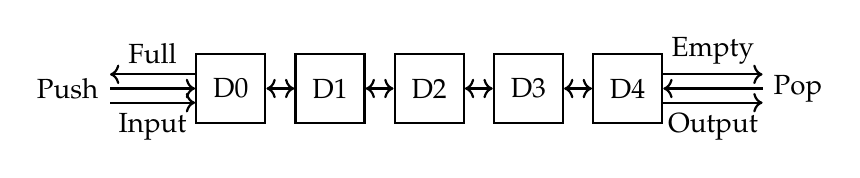
\begin{tikzpicture}[scale=0.9]
			% Draw FIFO boxes
			\foreach \i in {0,...,4} {
				\node[thick, rectangle,draw,minimum height=25, minimum width=25] (d\i) at (\i*1.4+0.5,0.5) {D\i};
			}
			\draw[<->, thick] (d0.east) -- (d1.west) {};
			\draw[<->, thick] (d1.east) -- (d2.west) {};
			\draw[<->, thick] (d2.east) -- (d3.west) {};
			\draw[<->, thick] (d3.east) -- (d4.west) {};
			
			% Arrows
			\draw[->, thick] ($(d0.west) + (-1.2,-0.2)$) -- ($(d0.west) + (0,-0.2)$) node[midway, below] {Input};
			\draw[->, thick] ($(d0.west) + (-1.2,0)$) -- ($(d0.west) + (0,0)$) node {};
			\draw node at ($(d0.west) + (-1.8,0)$){Push};
			\draw[<-, thick] ($(d0.west) + (-1.2,0.2)$) -- ($(d0.west) + (0,0.2)$) node[midway, above] {Full};
			
			\draw[->, thick] ($(d4.east) + (0,-0.2)$) -- ($(d4.east) + (1.4,-0.2)$) node[midway, below] {Output};
			\draw[<-, thick] ($(d4.east) + (0,0)$) -- ($(d4.east) + (1.4,0)$) node {};
			\draw node at ($(d4.east) + (1.9,0)$){Pop};
			\draw[->, thick] ($(d4.east) + (0,0.2)$) -- ($(d4.east) + (1.4,0.2)$) node[midway, above] {Empty};
			
		\end{tikzpicture}
	\end{center}
	
\end{frame}

\begin{frame}{Testing Levels}
	\begin{enumerate}
		\item \textbf{Unit Tests}
		\begin{itemize}
			\item Testing individual components in isolation
			\item Exercise basic units of functionality
		\end{itemize}
		
		\item \textbf{Integration Tests}
		\begin{itemize}
			\item Testing component interaction
			\item Compound units of functionality
		\end{itemize}
		
		\item \textbf{System Tests}
		\begin{itemize}
			\item Testing the complete system
			\item Use-case/user story tests
		\end{itemize}
		
		\item \textbf{Acceptance Tests}
		\begin{itemize}
			\item Testing by the client
		\end{itemize}
		
		\item Non-functional tests: Speed, size, documentation
	\end{enumerate}
\end{frame}

\begin{frame}{Testing Levels - Unit Tests}
	
	\begin{columns}
		\begin{column}{0.5\textwidth}
			\begin{itemize}
				\item Identify limited functionality
				\item Create tests covering the functionality
				\item Run and verified locally by developers
			\end{itemize}
		\end{column}
		\begin{column}{0.5\textwidth}
			\onslide<2->{
				\begin{center}
					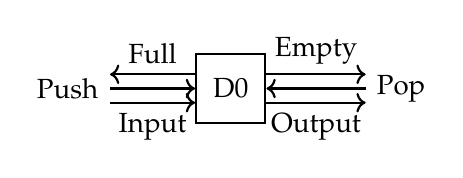
\begin{tikzpicture}[scale=0.9]
						
						\node[thick, rectangle,draw,minimum height=25, minimum width=25] (d0) at (0,0) {D0};
						
						% Arrows
						\draw[->, thick] ($(d0.west) + (-1.2,-0.2)$) -- ($(d0.west) + (0,-0.2)$) node[midway, below] {Input};
						\draw[->, thick] ($(d0.west) + (-1.2,0)$) -- ($(d0.west) + (0,0)$) node {};
						\draw node at ($(d0.west) + (-1.8,0)$){Push};
						\draw[<-, thick] ($(d0.west) + (-1.2,0.2)$) -- ($(d0.west) + (0,0.2)$) node[midway, above] {Full};
						
						\draw[->, thick] ($(d0.east) + (0,-0.2)$) -- ($(d0.east) + (1.4,-0.2)$) node[midway, below] {Output};
						\draw[<-, thick] ($(d0.east) + (0,0)$) -- ($(d0.east) + (1.4,0)$) node {};
						\draw node at ($(d0.east) + (1.9,0)$){Pop};
						\draw[->, thick] ($(d0.east) + (0,0.2)$) -- ($(d0.east) + (1.4,0.2)$) node[midway, above] {Empty};
						
					\end{tikzpicture}
				\end{center}
			}
		\end{column}
	\end{columns}
	\pause
	\textbf{FIFO Unit Tests (10):} Exercise: 3 mins
	\pause
	\begin{itemize}
		\item Initialized to empty
		\item On push becomes full \& !empty
		\item On pop becomes !full \& empty
		\item If empty, pop does nothing (pops zero?)
		\item If empty, push updates next pop
		\item If full, can pop
		\item If full, push doesn't change next pop
		\item Values pushed will be popped next cycle
		\item Can store indefinitely
		\item Can push and pop in simultaneously (forwarding?)
	\end{itemize}

\end{frame}

\begin{frame}{Testing Levels - Integration Tests}
	
	\begin{itemize}
		\item Identify common module interactions
		\item Create tests covering the functionality
		\item Run by either developers or dedicated testers
	\end{itemize}
	\pause
	\textbf{FIFO Tests (9):} Exercise: 5 mins
	\onslide<3->{
		\begin{itemize}
			\item Initialized to empty
			\item On push becomes !empty
			\item On pop becomes !full
			\item Pushed item will pop eventually
			\item List of items will pop in pushed order
			\item If full, can pop and push simultaneously
			\item Can store indefinitely
			\item Items get to the front without popping
			\item Two lists pushed eventually become one list
		\end{itemize}
	}
	\onslide<2->{
		\vspace{1em}
		\begin{center}
			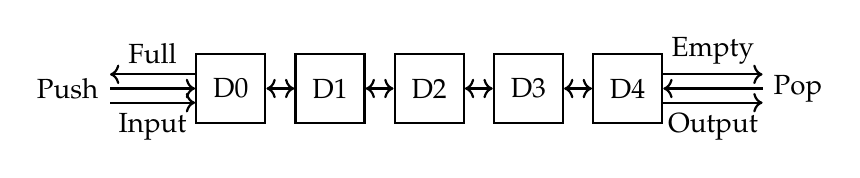
\begin{tikzpicture}[scale=0.9]
				% Draw FIFO boxes
				\foreach \i in {0,...,4} {
					\node[thick, rectangle,draw,minimum height=25, minimum width=25] (d\i) at (\i*1.4+0.5,0.5) {D\i};
				}
				\draw[<->, thick] (d0.east) -- (d1.west) {};
				\draw[<->, thick] (d1.east) -- (d2.west) {};
				\draw[<->, thick] (d2.east) -- (d3.west) {};
				\draw[<->, thick] (d3.east) -- (d4.west) {};
				
				% Arrows
				\draw[->, thick] ($(d0.west) + (-1.2,-0.2)$) -- ($(d0.west) + (0,-0.2)$) node[midway, below] {Input};
				\draw[->, thick] ($(d0.west) + (-1.2,0)$) -- ($(d0.west) + (0,0)$) node {};
				\draw node at ($(d0.west) + (-1.8,0)$){Push};
				\draw[<-, thick] ($(d0.west) + (-1.2,0.2)$) -- ($(d0.west) + (0,0.2)$) node[midway, above] {Full};
				
				\draw[->, thick] ($(d4.east) + (0,-0.2)$) -- ($(d4.east) + (1.4,-0.2)$) node[midway, below] {Output};
				\draw[<-, thick] ($(d4.east) + (0,0)$) -- ($(d4.east) + (1.4,0)$) node {};
				\draw node at ($(d4.east) + (1.9,0)$){Pop};
				\draw[->, thick] ($(d4.east) + (0,0.2)$) -- ($(d4.east) + (1.4,0.2)$) node[midway, above] {Empty};
				
			\end{tikzpicture}
		\end{center}
	}
\end{frame}

\begin{frame}{Test-Driven Development (TDD)}
	
	\textbf{What is TDD?}
	\begin{itemize}
		\item A software development approach where tests are written \textbf{before} the code
		\item Follows a short cycle: \textbf{Red → Green → Refactor}
	\end{itemize}
	\pause
	\vspace{1em}
	\textbf{TDD Cycle}
	\begin{enumerate}
		\item \textbf{Write a test} for a small piece of functionality
		\item \textbf{Run the test} – it should fail (Red)
		\item \textbf{Write the code} to make the test pass (Green)
		\item \textbf{Refactor} the code while keeping the test passing
	\end{enumerate}
	\pause
	\vspace{1em}
	\textbf{Benefits in Agile Design}
	\begin{itemize}
		\item Encourages modular, testable design
		\item Provides immediate feedback and confidence in changes
		\item Supports continuous integration and rapid iteration
	\end{itemize}
	
\end{frame}

\begin{frame}{Importance of Testable Design}
	
	\textbf{Why Design for Testability?}
	\begin{itemize}
		\item \textbf{Early Bug Detection:} Easier to identify and fix issues during development
		\item \textbf{Supports Automation:} Enables integration with CI
		\item \textbf{Improves Maintainability:} Modular and testable components are easier to update and refactor
		\item \textbf{Enables Agile Practices:} Prerequisite for iterative, feedback-driven development
	\end{itemize}
	\pause
	
	\textbf{In Digital Design Context:}
	\begin{itemize}
		\item Use of simulation testbenches for modules like FIFOs
		\item Design-for-Testability (DFT) features:
		\begin{itemize}
			\item Scan chains for test setup and verification
			\item Built-in self-test (BIST)
		\end{itemize}
		\item Clear separation of control and data paths for easier verification
	\end{itemize}
	
\end{frame}

\begin{frame}{Scan Chain - FIFO}
	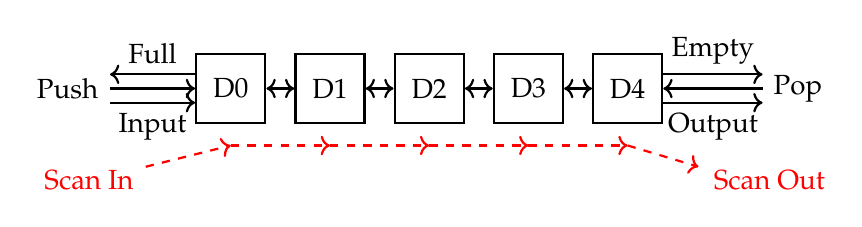
\begin{tikzpicture}[scale=0.9]
		% Draw FIFO boxes
		\foreach \i in {0,...,4} {
			\node[thick, rectangle,draw,minimum height=25, minimum width=25] (d\i) at (\i*1.4+0.5,0.5) {D\i};
		}
		
		% FIFO data flow arrows
		\draw[<->, thick] (d0.east) -- (d1.west);
		\draw[<->, thick] (d1.east) -- (d2.west);
		\draw[<->, thick] (d2.east) -- (d3.west);
		\draw[<->, thick] (d3.east) -- (d4.west);
		
		% Input/Output arrows
		\draw[->, thick] ($(d0.west) + (-1.2,-0.2)$) -- ($(d0.west) + (0,-0.2)$) node[midway, below] {Input};
		\draw[->, thick] ($(d0.west) + (-1.2,0)$) -- ($(d0.west) + (0,0)$);
		\node at ($(d0.west) + (-1.8,0)$){Push};
		\draw[<-, thick] ($(d0.west) + (-1.2,0.2)$) -- ($(d0.west) + (0,0.2)$) node[midway, above] {Full};
		
		\draw[->, thick] ($(d4.east) + (0,-0.2)$) -- ($(d4.east) + (1.4,-0.2)$) node[midway, below] {Output};
		\draw[<-, thick] ($(d4.east) + (0,0)$) -- ($(d4.east) + (1.4,0)$);
		\node at ($(d4.east) + (1.9,0)$){Pop};
		\draw[->, thick] ($(d4.east) + (0,0.2)$) -- ($(d4.east) + (1.4,0.2)$) node[midway, above] {Empty};
		
		% Scan chain path (dashed line)
		\draw[->, dashed, thick, red] ($(d0.south) + (-1.2,-0.6)$) -- ($(d0.south) + (0,-0.3)$);
		\draw[->, dashed, thick, red] ($(d0.south) + (0,-0.3)$) -- ($(d1.south) + (0,-0.3)$);
		\draw[->, dashed, thick, red] ($(d1.south) + (0,-0.3)$) -- ($(d2.south) + (0,-0.3)$);
		\draw[->, dashed, thick, red] ($(d2.south) + (0,-0.3)$) -- ($(d3.south) + (0,-0.3)$);
		\draw[->, dashed, thick, red] ($(d3.south) + (0,-0.3)$) -- ($(d4.south) + (0,-0.3)$);
		\draw[->, dashed, thick, red] ($(d4.south) + (0,-0.3)$) -- ($(d4.south) + (1,-0.6)$);
		
		% Scan input/output labels
		\node[below, red] at ($(d0.south) + (-2,-0.5)$) {Scan In};
		\node[below, red] at ($(d4.south) + (2,-0.5)$) {Scan Out};
	\end{tikzpicture}
	
	\pause
	\centering
	\vspace{3em}
	How does the scan chain change testing?
\end{frame}

\begin{frame}{Property-Based Testing (PBT)}
	
	\textbf{Why Property-Based Testing?}
	\begin{itemize}
		\item Many systems have an \textbf{infinite input space} — it's impractical to test all possible cases manually
		\item PBT helps uncover \textbf{classes of bugs} by generating a wide range of random, valid inputs
	\end{itemize}
	\pause
	\vspace{1em}
	\textbf{Core Strategy:}
	\begin{enumerate}
		\item \textbf{Identify a property} that should always hold (e.g., "push followed by pop returns the same value")
		\item \textbf{Define an input generator} that produces only valid inputs
		\item \textbf{Implement a reference (golden) model} to compare expected behavior
		\item \textbf{Run the test many times} with randomized inputs
	\end{enumerate}
	\pause
	\vspace{1em}
	\textbf{When a bug is found:}
	\begin{itemize}
		\item The failing input is \textbf{shrunk} to a minimal counterexample
		\item A new \textbf{unit or integration test} is created to capture and prevent regression
	\end{itemize}
	
\end{frame}

\begin{frame}[fragile]{Property-Based Testing in Chisel}
	\begin{itemize}
		\item Use of ScalaCheck for PBT
		\item Verifying hardware modules with randomized inputs
	\end{itemize}
	
	\vspace{1em}
	
	\begin{columns}
		\begin{column}{0.6\textwidth}
	\textbf{Example:}
	\begin{verbatim}
property("Push then pop") = 
forAll { (in: UInt) =>
	test(new FifoBlock()) { c =>
		c.io.push.poke(true.B)
		c.io.inputs.poke(in)
		c.clock.step()
		c.io.push.valid.poke(false.B)
		c.io.pop.poke(true.B)
		c.io.output.expect(in)
		c.clock.step()
		c.io.output.expect(0)
	}
}
	\end{verbatim}
	\end{column}
	\begin{column}{0.4\textwidth}
		\textbf{Key Points:}
		\begin{itemize}
			\item \texttt{forAll} generates random valid inputs
			\item The property asserts that pop returns the pushed value
			\item Failing cases are minimized and can be turned into regression tests
		\end{itemize}
	\end{column}
	\end{columns}
	
\end{frame}

\begin{frame}[fragile]{Example: Push/pop list}
	\scriptsize
	\begin{verbatim}
		property("FIFO preserves order of items") = 
		forAll { (depth: Int, inputs: List[Int]) =>
			whenever(depth > 0 && depth <= 32 && inputs.length <= depth) {
				test(new MyFifo(depth)) { c =>
					// Enqueue all elements
					for (in <- inputs) {
						c.io.push.poke(true.B)
						c.io.input.poke(in.U)
						c.clock.step()
					}
					while (c.io.empty.peek().litToBoolean) {
						c.clock.step()
					}
					
					// Dequeue and check order
					for (expected <- inputs) {
						c.io.pop.poke(true.B)
						c.io.output.expect(expected.U)
						c.clock.step()
					}
				}
			}
		}
	\end{verbatim}
	
\end{frame}

\begin{frame}[fragile]{\texttt{Arbitrary} and Shrinking}
	
	\textbf{Arbitrary}
	\begin{itemize}
		\item A type class used to define how to generate random values
		\item Default \texttt{Arbitrary} instances for common types (e.g., \texttt{Int}, \texttt{List[Int]})
		\item Define custom generators by creating your own \texttt{Arbitrary} instances
	\end{itemize}
	\pause
	\vspace{0.5em}
	\textbf{Example: Custom \texttt{Arbitrary} for Bounded Lists}
	\begin{verbatim}
implicit val smallListArb: Arbitrary[List[Int]] = 
Arbitrary {
	Gen.listOf(Gen.choose(0, 255)).suchThat(_.length <= 8)
}
	\end{verbatim}
	\pause
	\textbf{Shrinking}
	\begin{itemize}
		\item Tries to find the \textbf{smallest failing input}
		\item Helps identify minimal failures
	\end{itemize}
	\textbf{Tip:} Override default shrinking  using \texttt{Shrink}
	
\end{frame}

\begin{frame}[fragile]{Getting Started with ScalaCheck in Chisel}
\scriptsize
\begin{enumerate}
	
	\item \textbf{Add ScalaCheck to \texttt{build.sbt}:}
	\begin{verbatim}
		libraryDependencies += "org.scalacheck" %% "scalacheck" % "1.19.0" % Test
	\end{verbatim}
	
	\item \textbf{Import Required Packages:}
	\begin{verbatim}
		import org.scalacheck._
		import org.scalacheck.Prop.forAll
	\end{verbatim}
	
	\item \textbf{Create a ScalaCheck Property Class:}
	\begin{verbatim}
		class FifoProps extends Properties("FIFO") with ChiselScalatestTester {
			property("basic enqueue/dequeue") = forAll { (in: Int) =>
				test(new MyFifo(depth = 4)) { c =>
					...
				}
			}
		}
	\end{verbatim}
	
	\item \textbf{Run with \texttt{sbt test}}
	
\end{enumerate}

\end{frame}

\begin{frame}{Continuous Integration (CI): Motivation}
	
	\textbf{Tests are only useful if they are run!}
	
	\vspace{1em}
	\textbf{The Problem:}
	\begin{itemize}
		\item Developers may forget to run tests
		\item Different machines = inconsistent environments
		\item Tests can be time-consuming or complex
		\item As teams grow, ensuring everyone runs all tests becomes impractical
	\end{itemize}
	\pause
	\vspace{1em}
	\textbf{The Solution:}
	\begin{itemize}
		\item Use a CI server to automatically run tests on every change
		\item Integrate with version control (e.g., GitHub Actions, GitLab CI)
		\item Enforce test success before merging pull requests
	\end{itemize}
	
\end{frame}

\begin{frame}{Continuous Integration (CI): Benefits and Extras}
	\textbf{Key Benefits:}
	\begin{itemize}
		\item Developers don’t need to run all tests locally
		\item Tests run in a clean, consistent environment
		\item Regressions are caught \textbf{before} merging
		\item Ensures the \texttt{master} branch is always in a working state
	\end{itemize}
	
	\vspace{0.5em}
	\textbf{Additional Advantages:}
	\begin{itemize}
		\item Run performance or stress tests regularly
		\item Automate builds, documentation, and deployments
		\item Even useful for solo developers to avoid regressions
	\end{itemize}
	
	\vspace{0.5em}
	\textbf{CI Tools:}
	\begin{itemize}
		\item GitHub Actions, GitLab CI/CD, Jenkins, CircleCI, Travis CI
	\end{itemize}
	
\end{frame}

\begin{frame}[fragile]{Setting Up GitHub Actions CI for Chisel}
	\scriptsize
	
	\textbf{1. Create Workflow File:} \\
	In your repo, create the file: \texttt{.github/workflows/ci.yml}
	
	\pause
	\begin{columns}
		\begin{column}{0.5\textwidth}
			\textbf{2. Example \texttt{ci.yml} for Chisel Project:}
			\begin{verbatim}
name: CI
  on:
    pull_request:
    push:
  jobs:
    test:
    runs-on: ubuntu-latest
    steps:
      - name: Checkout
        uses: actions/checkout@v4
      - name: Setup JDK
        uses: actions/setup-java@v4
        with:
          distribution: temurin
          java-version: 11
      - name: Setup sbt launcher
        uses: sbt/setup-sbt@v1
      - name: Build and Test
        run: sbt test
			\end{verbatim}
		\end{column}
		\begin{column}{0.4\textwidth}
	
			\pause
			\textbf{3. Commit and Push:}
			\begin{itemize}
				\item Automatically run on each push or PR
				\item Check the \texttt{Actions} tab for results
			\end{itemize}
		\end{column}
	\end{columns}
	
\end{frame}

\begin{frame}{Lab session: Priority List}
	
	\textbf{Systolic Array Priority List}
	
	\begin{itemize}
		\item A \textbf{sorting structure} that maintains a list of key-value pairs in priority order
		\pause
		\item \textbf{Push:} Insert a new key and payload at the front of the array
		\item The key propagates through the array, \textbf{bubbling up} to its correct position
		\item \textbf{Pop:} Remove the smallest key and its payload from the end of the array
		\pause
		\item \textbf{Throughput:} One pop every 2 cycles (after initial latency)
		\item \textbf{Applications:} Used in high-speed systems like \textbf{network routers}
		\item \textbf{Trade-offs:}
		\begin{itemize}
			\item Very low latency
			\item High hardware cost (area and power)
			\item Highly parallel and pipelined
		\end{itemize}
		\pause
		\item \textbf{Configurable:} Key size, payload size, and array length
	\end{itemize}
	
\end{frame}

\begin{frame}{Commands and Configuration}
	
	\textbf{Supported Commands:}
	\begin{itemize}
		\item \texttt{IDLE} – Do nothing
		\item \texttt{PUSH} – Insert a key/payload pair into the front of the array
		\item \texttt{POP} – Remove the smallest key/payload pair from the end
		\item \texttt{PUSH/POP} – Simultaneously insert a new pair and remove the smallest
	\end{itemize}
	
	\pause
	\vspace{0.5em}
	\textbf{Design Requirements:}
	\begin{itemize}
		\item \textbf{Configurable parameters:}
		\begin{itemize}
			\item \texttt{keyWidth} – Bit width of the key (used for sorting)
			\item \texttt{valueWidth} – Bit width of the payload
			\item \texttt{depth} – Number of stages in the systolic array
		\end{itemize}
		\item \textbf{Modular design:} Each stage compares and forwards data
		\item \textbf{Testable:} Design should support unit and integration testing
	\end{itemize}
	
\end{frame}

\begin{frame}{Systolic Array Priority List: Node}
	\centering
	
	\begin{center}
		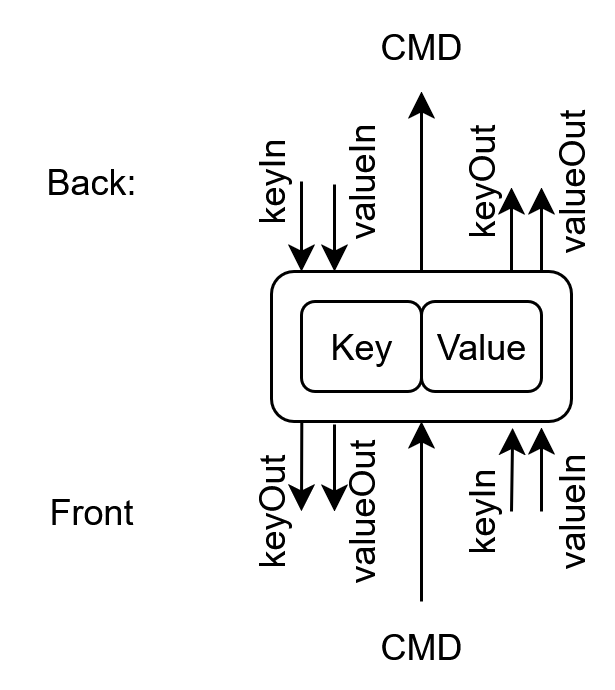
\includegraphics[width=0.6\textwidth]{images/systolic node.png}
	\end{center}
\end{frame}

\begin{frame}{Systolic Array Priority List}
\centering

\begin{center}
	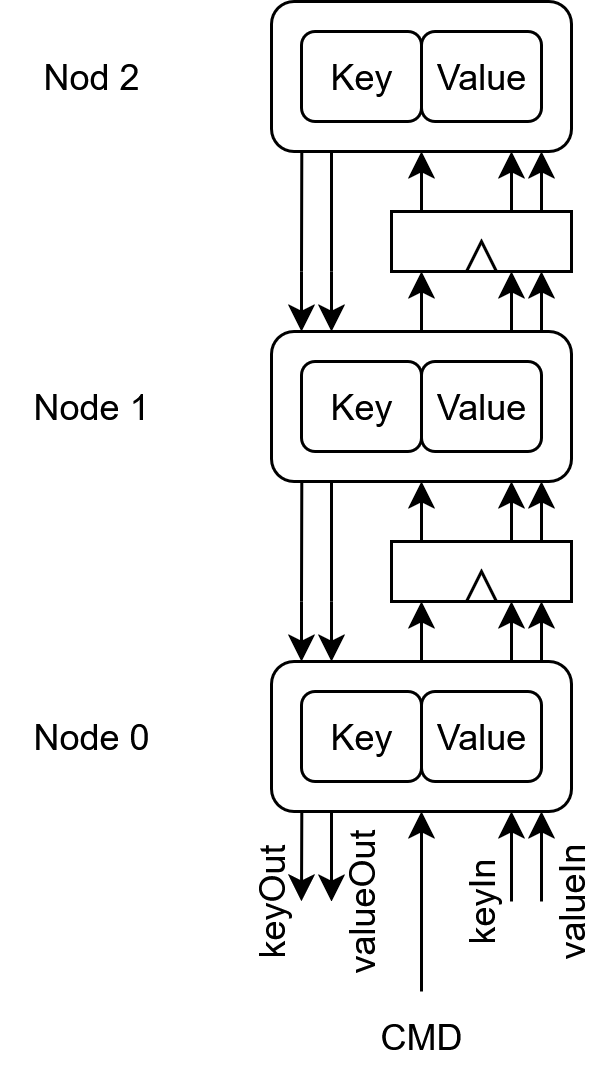
\includegraphics[width=0.4\textwidth]{images/prio-list.png}
\end{center}
\end{frame}

\begin{frame}{Testing the Priority List}
	
	\textbf{How should this be tested?}
	\pause
	\begin{itemize}
		\item \textbf{Unit Tests:} 
		\begin{itemize}
			\item Test individual array elements (stages) for correct compare-and-forward behavior
		\end{itemize}
		
		\item \textbf{Integration Tests:}
		\begin{itemize}
			\item Validate full array behavior across PUSH/POP operations
			\item Ensure keys bubble correctly and throughput matches expectations
		\end{itemize}
		
		\item \textbf{Property-Based Tests:}
		\begin{itemize}
			\item \textbf{Push-Pop Consistency:} Every pushed value should eventually be popped
			\item \textbf{Sorted Output:} Popped values should be in ascending key order
			\item \textbf{Idle Preservation:} IDLE cycles should not lose or corrupt data
			\item \textbf{Stable Sorting:} Equal keys should preserve insertion order
		\end{itemize}
	\end{itemize}
	
\end{frame}

\begin{frame}{Extension: Grouped Value Support}
	
	\textbf{New Requirements:}
	\begin{itemize}
		\item Values must be tracked in \textbf{groups}—each key may have multiple associated values
		\item Each \texttt{PUSH} command may insert a \textbf{variable number of values}
		\item Newly pushed values must \textbf{merge} with existing values for the same key
		\item System should be \textbf{configurable} in terms of maximum pair lengths
	\end{itemize}
	
	\vspace{0.5em}
	\textbf{Extended Commands:}
	\begin{itemize}
		\item \texttt{Push(0)} – No operation
		\item \texttt{Pop(0)} – Pop lowest key and its value group
		\item \texttt{Push(x)} – Push \texttt{x} values with a given key
		\item \texttt{Pop(x)} – Pop lowest key group, then push \texttt{x} values with a new key
	\end{itemize}
	
\end{frame}

\begin{frame}{Summary}
	\begin{itemize}
		\item Testing is an integral part of agile development
		\item Test-driven development aids fast iteration and cooperation
		\item Property-based testing increases test quality
		\item Continuous integration ensures code quality is maintained
		\item Lab session: Priority List
	\end{itemize}
\end{frame}

\end{document}

\begin{frame}[fragile]{Title}
\begin{itemize}
\item abc
\end{itemize}
\end{frame}
